% Section content template for individual Educative lessons
% This file contains the actual content for a specific section
% Generated from Educative API section content

% Section: Activity Diagram for the Meeting Scheduler
% Section ID: 5955594525868032
% Section Slug: activity-diagram-for-the-meeting-scheduler
% Generated: 2025-12-12T13:06:45.037256

Activity diagrams are a great way to visualize the flow of messages from one activity to another in the system. There can be different activity diagrams that we can create for our meeting scheduler. In this lesson, we will create activity diagrams for the following two activities:

\begin{itemize}
\item
\protect\phantomsection\label{Fb5heVTUO4vB6J6-2akTj}
Schedule a meeting.
\item
\protect\phantomsection\label{zMlhwk46V1KYyip-U9e6V}
\textbf{Activity challenge:} Respond to an invite.
\end{itemize}

\subsection{Schedule meeting}\label{GSDBjuDpgq4ks__FC9WIR}
\\
The following states and actions will be involved in this activity diagram.

\subsubsection{States}\label{jI0Te_D70WuELbMrQkpY4}
\\
\textbf{Initial state:~} The user opens the calendar.
\\
\textbf{Final state:~} The notification and meeting details are sent to all the invited participants.

\subsubsection{Actions}\label{RpmGoluXnwb00TKn39xiB}
\\
The user opens the calendar and selects an available slot. The user books a meeting room, and the meeting details are sent to all invited users.

\begin{figure}[htbp]
 \centering
 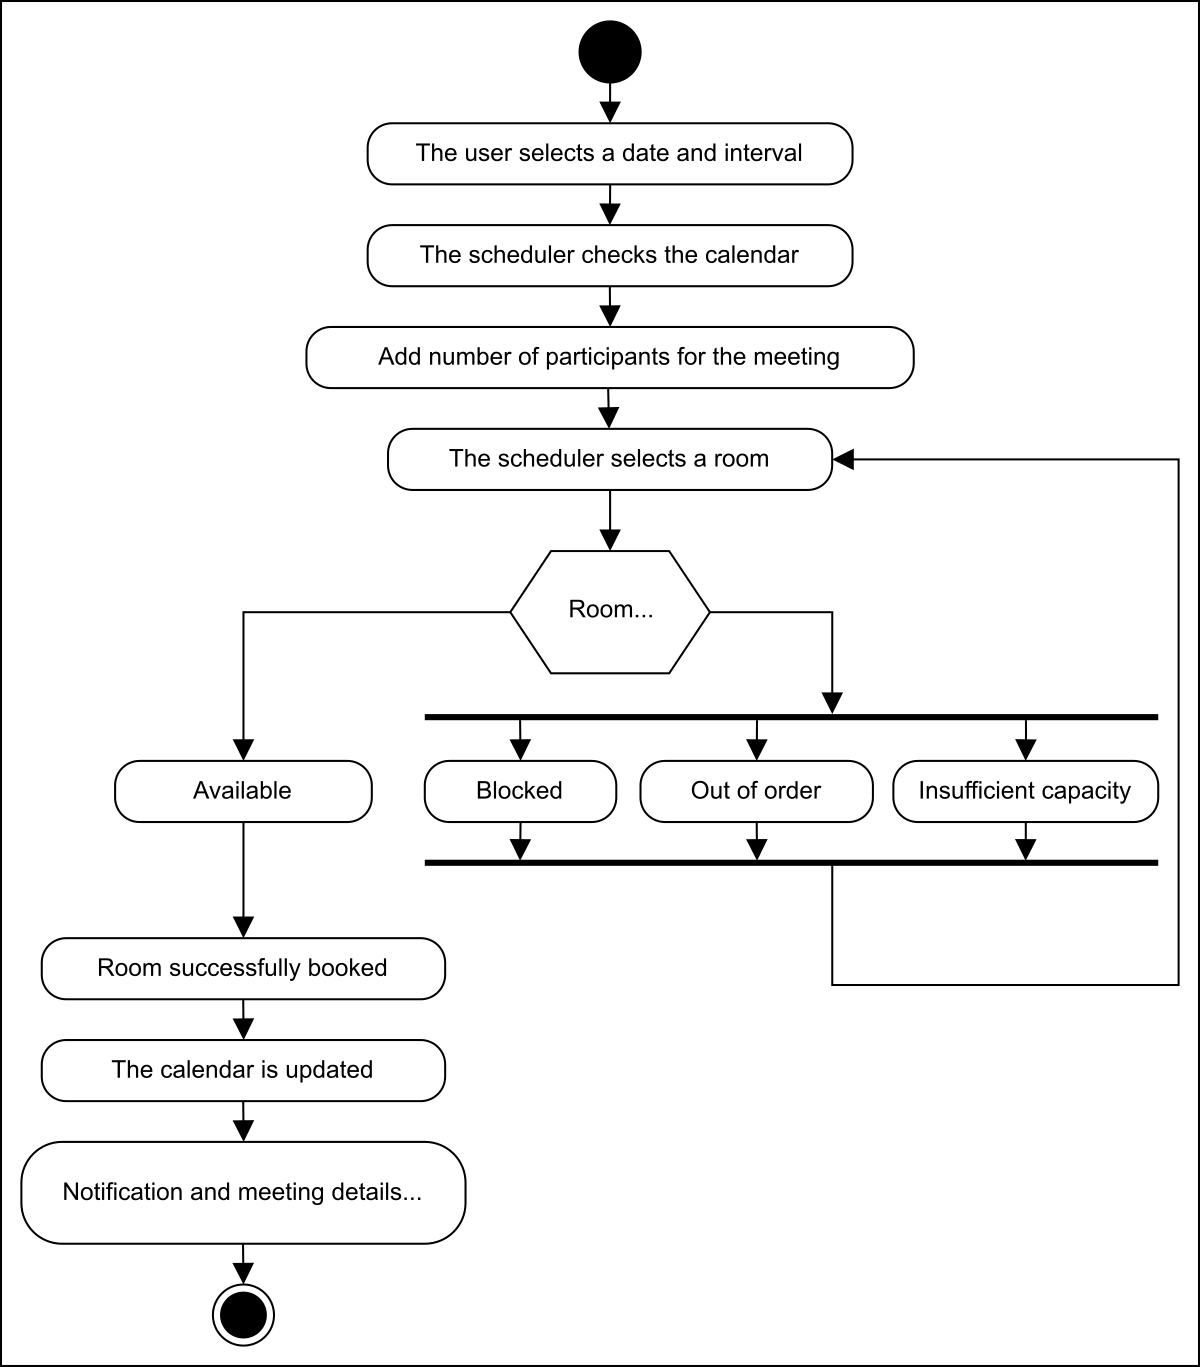
\includegraphics[width=0.5\textwidth]{Images/chapter_13/section_5955594525868032/6567554383609856.png}
 \caption{The activity diagram for a user scheduling a meeting}
\end{figure}

\subsection{Activity challenge: Respond to an invite}\label{liO8EB2r6oceODjMO-5Tq}
\\
You'll help us create an activity diagram of a person responding to an invite.
\\
A skeleton of the activity diagram is given below:

\begin{figure}[htbp]
 \centering
 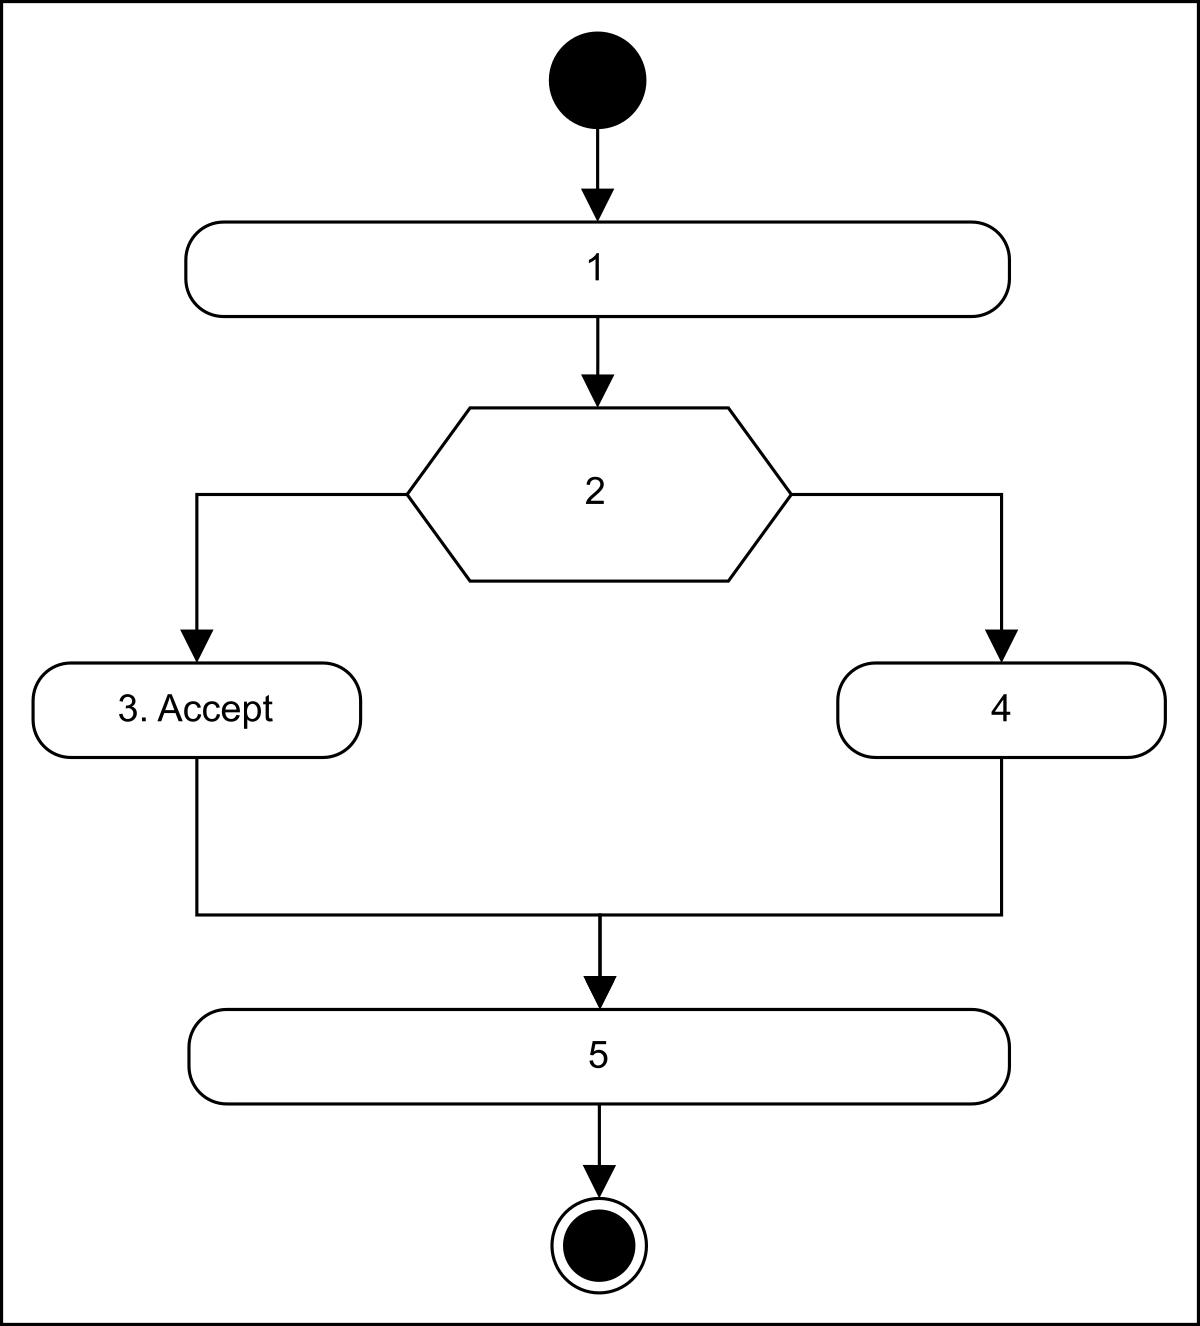
\includegraphics[width=0.5\textwidth]{Images/chapter_13/section_5955594525868032/6640117752266752.png}
 \caption{The activity diagram for a user responding to an invite}
\end{figure}

Notice that the actions in the diagram above are numbered from 1 to 6. The slots below represent the activities, and the arrows represent the flow from one activity to another.
\\
Can you rearrange the slots below in the correct order they should appear in the activity diagram above?
\begin{quote}
\textbf{Note:} If you're stuck, click the ``Show Solution'' button.
\end{quote}

Alternatively, you can click the ``Show complete diagram'' button below to see the complete activity diagram.

We've looked at some of our meeting scheduler's activity diagrams. In the next lesson, we will present the code for our designed classes in some of the most popular languages.

% End of section content